%%%%%%%%%%%%%%%%%%%%%%%%%%%%%%%%%%%%%%%%%%%%%%%%%%%%%%%%%%%%%%%%%%%%%%%%%%%%%%%%
%Tutorial slides on Python.
%
% Author: FOSSEE 
% Copyright (c) 2009, FOSSEE, IIT Bombay
%%%%%%%%%%%%%%%%%%%%%%%%%%%%%%%%%%%%%%%%%%%%%%%%%%%%%%%%%%%%%%%%%%%%%%%%%%%%%%%%

\documentclass[14pt,compress]{beamer}
%\documentclass[draft]{beamer}
%\documentclass[compress,handout]{beamer}
%\usepackage{pgfpages} 
%\pgfpagesuselayout{2 on 1}[a4paper,border shrink=5mm]

% Modified from: generic-ornate-15min-45min.de.tex
\mode<presentation>
{
  \usetheme{Warsaw}
  \useoutertheme{infolines}
  \setbeamercovered{transparent}
}

\usepackage[english]{babel}
\usepackage[latin1]{inputenc}
%\usepackage{times}
\usepackage[T1]{fontenc}

% Taken from Fernando's slides.
\usepackage{ae,aecompl}
\usepackage{mathpazo,courier,euler}
\usepackage[scaled=.95]{helvet}

\definecolor{darkgreen}{rgb}{0,0.5,0}

\usepackage{listings}
\lstset{language=Python,
    basicstyle=\ttfamily\bfseries,
    commentstyle=\color{red}\itshape,
  stringstyle=\color{darkgreen},
  showstringspaces=false,
  keywordstyle=\color{blue}\bfseries}

%%%%%%%%%%%%%%%%%%%%%%%%%%%%%%%%%%%%%%%%%%%%%%%%%%%%%%%%%%%%%%%%%%%%%%
% Macros
\setbeamercolor{emphbar}{bg=blue!20, fg=black}
\newcommand{\emphbar}[1]
{\begin{beamercolorbox}[rounded=true]{emphbar} 
      {#1}
 \end{beamercolorbox}
}
\newcounter{time}
\setcounter{time}{0}
\newcommand{\inctime}[1]{\addtocounter{time}{#1}{\tiny \thetime\ m}}

\newcommand{\typ}[1]{\lstinline{#1}}

\newcommand{\kwrd}[1]{ \texttt{\textbf{\color{blue}{#1}}}  }

% Title page
\title{Python for Scientific Computing : Large Scale Data Processing}

\author[FOSSEE] {FOSSEE}

\institute[IIT Bombay] {Department of Aerospace Engineering\\IIT Bombay}
\date{}

% DOCUMENT STARTS
\begin{document}

\begin{frame}
  \maketitle
\end{frame}

\begin{frame}
  \frametitle{About the Session}
  \begin{block}{Goal}
    We read and process large data file to solve a problem.
  \end{block}
  \begin{block}{Checklist}
    \begin{itemize}
    \item sslc.txt
  \end{itemize}
  \end{block}
\end{frame}

\begin{frame}
  \frametitle{Structure of the file}
  Understanding the structure of sslc.txt
  \begin{itemize}
    \item 180,000 lines. 
    \item Each line in the file has a student's details(record)
    \item Each record consists of fields separated by ';'
  \end{itemize}
\end{frame}

\begin{frame}
  \frametitle{Structure of the file \ldots}
\emphbar{A;015163;JOSEPH RAJ S;083;042;47;AA;72;244;;;}
  Each record consists of:
  \begin{itemize}
    \item Region Code : 'A'
    \item Roll Number : '015163'
    \item Name : 'JOSEPH RAJ S'
    \item Marks of 5 subjects: English(083), Hindi(042), Maths(47), Science(AA), Social(72)
    \item Total marks : 244
    \item Pass/Fail (P/F) : ' '
    \item Withheld (W) : ' '
  \end{itemize}
\end{frame}

%% \begin{frame}
%%   \frametitle{Statistical Analysis: Problem statement}
%%   1. Read the data supplied in the file \emph{sslc.txt} and carry out the following:
%%   \begin{block}{}
%%     Draw a pie chart representing proportion of students who scored more than 90\% in each region in Science.    
%%   \end{block}
%% \end{frame}

\begin{frame}
  \frametitle{Problem statement: explanation}
    \emphbar{Draw a pie chart representing proportion of students who scored more than 90\% in each region in Science.}
    \begin{columns}
    \column{5.25\textwidth}
    \hspace*{.5in}
    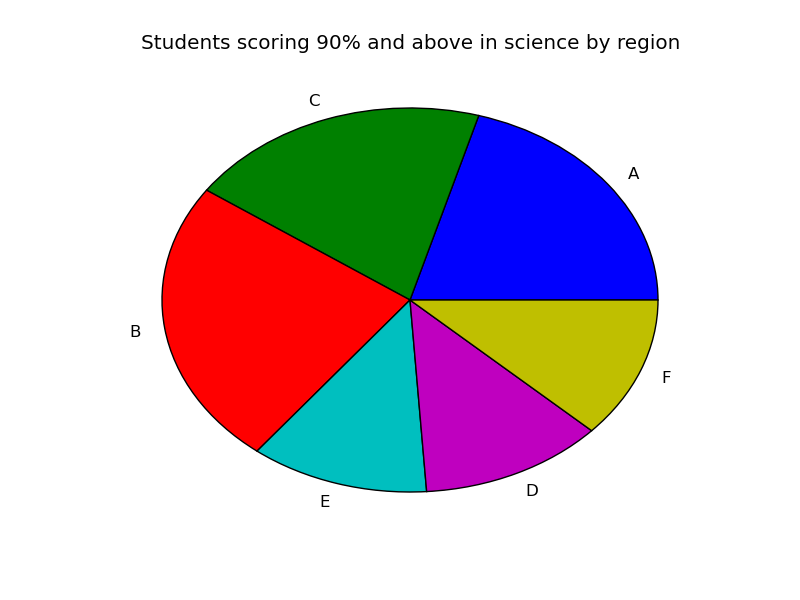
\includegraphics[height=2.6in, interpolate=true]{data/science}
    \column{0.8\textwidth}
\end{columns}
\end{frame}

\begin{frame}
  \frametitle{Machinery Required}
  \begin{itemize}
    \item File reading 
    \item Dictionaries 
    \item Parsing 
    \item Plot 
  \end{itemize}
\end{frame}

\begin{frame}[fragile]
  \frametitle{Summary}
  \begin{block}{Data processing}
    \begin{itemize}
    \item Dictionaries
    \item String parsing
    \item Pie charts
    \end{itemize}  
  \end{block}
\end{frame}

\begin{frame}
  \frametitle{Thank you!}  
  \begin{block}{}
  This session is part of \textcolor{blue}{FOSSEE} project funded by:
  \begin{center}
    \textcolor{blue}{NME through ICT from MHRD, Govt. of India}.
  \end{center}  
  \end{block}
\end{frame}

\end{document}
